%\documentclass[referee]{aa} % for a referee version
%\documentclass[onecolumn]{aa} % for a paper on 1 column  
%\documentclass[longauth]{aa} % for the long lists of affiliations 
%\documentclass[letter]{aa} % for the letters 
\documentclass{aa}

\usepackage{txfonts}
\usepackage{natbib}

\usepackage{graphicx}

\usepackage{color}
\usepackage{hyperref}
\hypersetup{colorlinks=true,allcolors=[rgb]{0,0,0.8}}


\usepackage{showyourwork}

% the three lines suppress the hyperref 'link empty' warnings
% explanation at: https://tex.stackexchange.com/questions/345764/journal-class-shows-package-hyperref-warning-suppressing-link-with-empty-targe
\makeatletter
\renewcommand*\aa@pageof{, page \thepage{} of \pageref*{LastPage}}
\makeatother

\usepackage{xspace}

\newcommand{\ktwo}{\textit{K2}}
\newcommand{\kms}{km~s$^{-1}$\xspace}
\newcommand{\ms}{m~s$^{-1}$}
\newcommand{\gcc}{g~cm$^{-3}$}
\newcommand{\masyr}{mas~yr$^{-1}$}
\newcommand{\err}{\textit{$\pm$}}
\newcommand{\teff}{$T_\mathrm{eff}$}
\newcommand{\msun}{$M_\odot$}
\newcommand{\rsun}{$R_\odot$}
\newcommand{\lsun}{$L_\odot$}
\newcommand{\rhosun}{$\rho_\odot$}
\newcommand{\mstar}{$M_*$}
\newcommand{\rstar}{$R_*$}
\newcommand{\lstar}{$L_*$}
\newcommand{\rearth}{$R_\oplus$}
\newcommand{\vrad}{$v_{R}$}
\newcommand{\pmra}{$\mu_{\alpha}$}
\newcommand{\pmdec}{$\mu_{\delta}$}

\newcommand{\rhostar}{$\rho_*$}
\newcommand{\mjup}{$M_\mathrm{Jup}$}
\newcommand{\galex}{\textit{GALEX}}
\newcommand{\gaia}{\textit{Gaia}}
\newcommand{\kepler}{\textit{Kepler}}
\newcommand{\spitzer}{\textit{Spitzer}}
\newcommand{\ktwosc}{\textsc{k2sc}}
\newcommand{\ktwosff}{\textsc{k2sff}}
\newcommand{\hipparcos}{\textit{Hipparcos}}
\newcommand{\tess}{\textit{TESS}}
\newcommand{\emcee}{\textsc{emcee}}
\newcommand{\python}{\textsc{python}}


\begin{document} 

   \title{The eclipse of ASASSN-21qj}

   \author{M. Kenworthy
          \inst{1}
          \and
          Arttu Sainio
          \inst{2}
          \and
          Eric E. Mamajek
          \inst{3}
          \and
          Joeseph Masiero
          \inst{4}
          \and 
          Amy Mainzer
          \inst{4}
          \and
          Joeseph (Davy) Kirkpatrick
          \inst{4}
          \and 
          Grant M. Kennedy
          \and
          Ludmila Carone
          \and
          NEOWISE authorship list
          \inst{4}
          \and
          AAVSO observers
          \and
          St\'{e}phane Charbonnel
          \and
        Olivier Garde
        \and
        Pascal Le D\^{u}
        \and
        Lionel Mulato
        \and
        Thomas Petit
          }

   \institute{Leiden Observatory, University of Leiden,
   PO Box 9513, 2300 RA Leiden, The Netherlands\\
   \email{kenworthy@strw.leidenuniv.nl}
         \and
             Arttu's address ...\\
    \and
    JPL
    \and
    Caltech/IPAC, 1200 E California Blvd, Mail Code 100-22, Pasadena, CA 91125, USA
    \and
    NEOWISE
    \and
    AAVSO people
    \and
    Space Research Institute, Austrian Academy of Sciences, Schmiedlstrasse 6, A-8042 Graz, Austria
}
   \date{Received XXXX; accepted XXXX}

% \abstract{}{}{}{}{} 
% 5 {} token are mandatory
 
  \abstract
  % context heading (optional)
  % {} leave it empty if necessary  
   {Collisions occur between planetessimals that generate debris disks through collisional cascades.}
  % aims heading (mandatory)
   {We analyze the dust and size distribution of the eclipse seen towards ASASSN-21qj.}
  % methods heading (mandatory)
   {Fit the light curve from three different colours to determine the particle size and distribution.}
  % results heading (mandatory)
   {The eclipse is coloured, indicating dust.
   %
   The dust has a lower limit mass of XXXX Earths, eclipse has a duration of XXXX days.}
  % conclusions heading (optional), leave it empty if necessary 
   {}

   \keywords{giant planet formation --
                $\kappa$-mechanism --
                stability of gas spheres
               }

   \maketitle
%
%-------------------------------------------------------------------

   \section{Introduction}

Terrestrial planets are thought to be built up by the quasi-periodic accretion of planetary embryos that generate a significant amount of ejected material.
%
The Earth's moon is believed to have formed from the resulting aftermath of a collision in the early Solar system.
%
Sudden increases of infrared flux from systems known to host debris disks indicate that this is a stochastic process that can occur on timescales of a few months or less.
%
Models of these impacts and the subsequent evolution of the dust clouds have been modeled \citep{Jackson12,Jackson14} and have been seen ar IR wavelengths \citep{Su19,Su22}

   The star (Gaia EDR3 source 5539970601632026752 at RA=08:15:23.2996, DEC=-38:59:23.304, $d\sim 556$ pc, G=13.4 mag, BP-RP=0.8 mag) underwent a sudden dimming event in December 2021, which was announced by \citet{RizzoSmith21} and assigned the identifier ASASSN-21qj.
   %
   The star has subsequently maintained rapidly fluctuating photometry through to August 2022 \citep{RizzoSmith22} and has been monitored intensively by the AAVSO observers and the LCOGT network of telescopes.
   %
   It had previously shown no significant stellar variation in the optical bands for 2300 days as reported in \citet{RizzoSmith21}.
   %
   Searches through other photometric archives showed no other significant changes in the optical bands before this epoch.
   %
   The wide field infrared satellite WISE has photometric imaging from 3.8 microns (band W1) through to 25 microns (band W4), and the NEOWISE survey has photometry for bands W1 and W2 for this star.
   %
   This star showed a significant brightening of 0.7 magnitudes in W1 and 0.8 magnitudes in W2 between two observing epochs (65000 MJD and 65120 MJD), and the IR color of the star had changed from W1-W2=0.0 to 1.2, but no significant changes in flux in the optical bands were seen during this time.
   %
   Some 900 days later, the dimming was seen in the optical, and the absorption is larger at shorter optical wavelengths.
   %
   These observations are all consistent with an event that generated a significant amount of sub-micron dust which subsequently started to transit the stellar disk.

   We hypothesise that there was a collision between one or more rocky bodies in the system which generated a significant amount of dust, which has then subsequently begun to transit the star.
   %
   This is consistent with a late type impact between a planet and large asteroid, similar to the one that generated the Earth/Moon system.

   The structure of our paper is as follows: the analysis of the star is given in Section~\ref{sec:star}, the observations are detailed in Section~\ref{sec:obs}, and we make an estimate of the physical parameters of the hypothesised dust cloud in Section~\ref{sec:dustcloud}.
   %
   We then place this model in the context of planet formation in Section~\ref{sec:discussion} and summarise the paper in Section~\ref{sec:conclusion}.


Statistical distributions of ejecta masses from collision in \citet{Crespi21}.

Planetary embryo collisions and wiggly disks.... \citet{Watt21}.

\section{Properties of the star}\label{sec:star}

The properties of ASASSN-21qj (Gaia EDR3 source 5539970601632026752) are listed in Table~\ref{tab:Stellarprop}.

\begin{table}
    \centering
    \caption{ Properties of ASASSN-21qj}
    \begin{tabular}{@{}lcc@{}}
    \hline\hline
Property                               & Value                     & Ref.  \\
        \hline
         $\alpha_{ICRS}$, J2000 {[}hh mm ss{]}  & 08:15:23.30              & 1     \\
         $\delta_{ICRS}$, J2000 {[}dd mm ss{]}  & -38:59:23.3              & 1     \\
         $\mu_{\alpha}$ {[}mas yr$^{-1}${]}     & $-9.692\pm0.012$          & 1     \\
         $\mu_{\delta}$ {[}mas yr$^{-1}${]}     & $7.349\pm0.012$          & 1     \\
         $\varpi$ {[}mas{]}                     & $1.763\pm0.011$         & 1     \\
         Distance {[}pc{]}                      & $XXXX^{+6.7}_{-5.9}$     & 2     \\ 
        \hline
         $G$ {[}mag{]}                          & $13.371\pm XXXX$        & 1     \\
         $G_{BP}-G_{RP}$ {[}mag{]}              & $0.815\pm XXXX$        & 1     \\
         $G_{BP}$ {[}mag{]}                     & $13.697\pm XXXXX$        & 1     \\
         $G_{RP}$ {[}mag{]}                     & $12.882\pm XXXXX$        & 1     \\
%         $J$ {[}mag{]}                          & $12.897\pm0.026$          & 3     \\
%         $H$ {[}mag{]}                          & $12.431\pm0.024$          & 3     \\
%         $K$ {[}mag{]}                          & $12.321\pm0.024$          & 3     \\
%         $u$ (AB) {[}mag{]}                     & $17.63\pm0.02$            & 4     \\
%         $g$ (AB) {[}mag{]}                     & $16.096\pm0.008$          & 4     \\
%         $r$ (AB) {[}mag{]}                     & $16.69\pm0.02$            & 4     \\
%         $i$ (AB) {[}mag{]}                     & $14.123\pm0.005$          & 4     \\
%         $z$ (AB) {[}mag{]}                     & $14.832\pm0.011$          & 4     \\
        \hline
         $R_*$ [\rsun{}]                        & $1.009\pm0.030$           & 5     \\
%         $M_*$ [$M_{\odot}$]                    & $0.85\pm0.02$             & 5     \\
         {[}Fe/H{]} [dex]                       & $0.0\pm0.23$               & 5     \\
         log\,$g$ [log$_{10}$ cm\,s$^{-2}$]     & $4.5\pm0.25$               & 5     \\
         \teff{} [K]                            & $5900\pm74$               & 5     \\
%         $f_{bol}$ [10$^{-11}$ erg s$^{-1}$]    & $5.288\pm0.130$           & 5     \\
%         $m_{bol}$ [mag]                        & $14.194\pm0.027$          & 5     \\
         $m_{bol}$ [mag]                        & $13.39\pm0.02$           & 5     \\
%         $L_{bol}$ [$L_{\odot}$]                & $0.046\pm0.013$         & 5     \\
         log($L/L_{bol}$) [dex]                 & $0.046\pm0.013$        & 5     \\
         
        \hline
    \end{tabular}
    \tablefoot{References:
    (1) Gaia EDR3 \citep{Brown21},
    (2) \citet{BailerJones21},
    (3) 2MASS \citep{Cutri03},
    (4) SDSS DR8,
    (5) this work (EEM fits)
    }
    \label{tab:Stellarprop}
\end{table}

% Including IR WISE photometry
%was forcing it to lower metallicity ([Fe/H] ~ -0.5-1), cooler (~Sun) fits. Fits also favor low reddening values ($A_v\sim 0.05$). 
%Similar to Alpha Cen A, but ~solar metallicity seems OK now. Almost exactly 1 Rsun! 

%Best parameters as of 1/2/2022 (see below from VOSA fit) 
%Teff = 5900 +- 74 K
%log(L/Lsun) = 0.046+-0.013 
%Av = 0.05+-0.03
%mbol = 13.39+-0.02 (apparent)
%logg = 4.5+-0.25
%[M/H] = 0.0+-0.23 
%Rad = 1.009 +- 0.030 Rsun


\begin{figure}
   \centering
   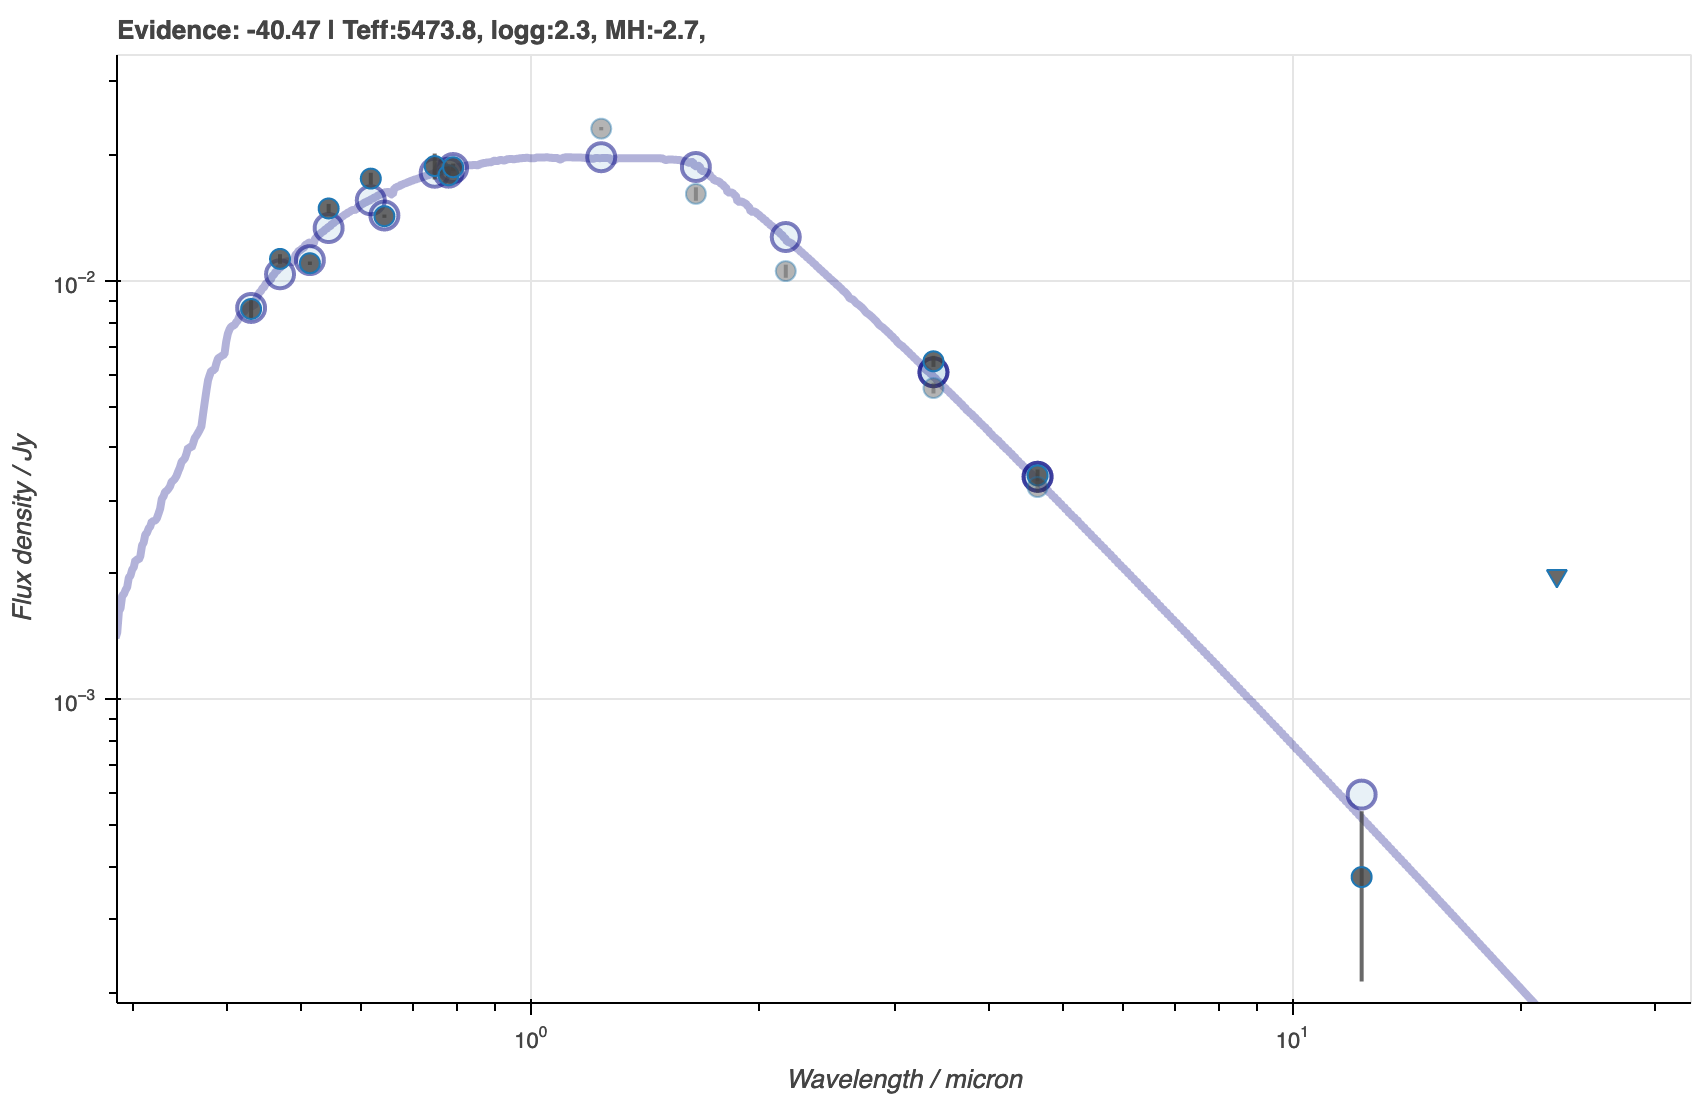
\includegraphics[width=\hsize]{figures/asassn-21qj-gmk-sed-fit.png}
      \caption{VOSA fit to photometry of ASAS-SN J0815 by gmk}
         \label{fig:sed}
\end{figure}


\begin{figure}
   \begin{centering}
   \includegraphics[width=\hsize]{figures/filter_curves.pdf}
      \caption{Filter curves for all telescopes and filters used to observe ASASSN-21qj.}
      \label{fig:allfilters}
      \script{plot_filter_curves.py}
      \end{centering}
\end{figure}



\begin{figure}
   \begin{centering}
   \includegraphics[width=\hsize]{figures/mie_single.pdf}
      \caption{Mie test.}
      \label{fig:mietest}
      \script{plot_mie_single.py}
      \end{centering}
\end{figure}




\begin{figure*}
   \begin{centering}
   \includegraphics[width=\textwidth]{figures/eclipse_overview2.pdf}
      \caption{Photometry from the optical bands of the eclipse.
      %
The different telescopes and filters are indicated in the legend.
%
Each light curve is offset vertically by 0.8.
              }
        \label{fig:eclipse_overview}
        \script{plot_eclipse_overview2.py}
    \end{centering}
\end{figure*}



\subsection{Possible multiplicity in the  system}

ASASSN-21qj (Gaia DR3 5539970601632026752 = 2MASS J08152329-3859234) has a neighbor (Gaia DR3 5539970597334497024= 2MASS J08152298-3859244) a few arcseconds away for which we checked to see if it could plausibly be a physical companion.
%
Based on the Gaia EDR3 mean ICRS position for epoch 2016.0, the visual companion lies at a separation $\rho$ = $3738.243\pm0.062$ mas and at position angle $\theta$ = $249^{\circ}.977$.
%
Their parallaxes ($\varpi$ = $1.7631\pm0.0112$ mas vs. $1.4711\pm0.0523$ mas) differ by 5.5$\sigma$ and proper motions ($\mu_{\alpha} = -9.692\pm0.012$, $\mu_{\delta} = 7.349\pm0.012$ \masyr\, vs. $\mu_{\alpha} = -0.114\pm0.055$, $\mu_{\delta} = 6.419\pm0.053$ \masyr) differ by a factor of 2.
%
If the two stars are at the parallactic distance of ASASSN-21qj
\citep[$d$ = 552.4 pc;][]{BailerJones21}, then their difference in proper motion ($\Delta\mu$ = $9.623\pm0.056$ \masyr) translates to a difference in tangential velocity of $\Delta V_{tan}$ = $25.37\pm0.21$ \kms.
%
The velocity difference is considerable given the projected separation of 2079\,au.
%
Using Kepler's 3rd law, and assuming the observed separation corresponded
to the semi-major axis, and the observed $\Delta V_{tan}$ corresponded to the full orbital velocity, these quantities would predict a minimum system mass of $>$1509 Msun.
%
Based on the implausible estimated dynamical mass inferred from the observed separation and difference in tangential velocities, we conclude that the visual companion Gaia DR3 5539970597334497024 (2MASS J08152298-3859244) is an interloper
unrelated to ASASSN-21qj.

\section{Observations}\label{sec:obs}
An overview of all the photometry is presented in Figure~\ref{fig:allphot}.




\subsection{ASAS-SN photometry}

The beginning of the eclipse was identified in \citet{RizzoSmith21} through the ASAS-SN survey.
%

\subsection{ROAD Photometry}


\subsection{NEOWISE photometry}

The NEOWISE photometry is presented with the ASASSN $q$ light curve in Figure~\ref{fig:wisephot}.

\begin{figure*}
\begin{centering}
\includegraphics[width=\textwidth]{figures/all_photometry.png}
\caption{NEOWISE $W1$ and $W2$ photometry of the star, with the WISE color in the lowest panel.
%
The $NEOWISE$ color changes from colourless to very red, which fades back towards colourless over $\sim 500$ days.
}
\label{fig:wisephot}
\script{plot_all_photometry.py}
\end{centering}
\end{figure*}


\begin{figure*}
\begin{centering}
\includegraphics[width=\textwidth]{figures/stellar_lomb_scargle.pdf}
\caption{ASASSN photometry of ASASSN-21qj and the Lomb Scargle periodograms of the photometry in and out of the eclipse.
%
The blue and orange shaded regions in the top panel indicate the range of epochs put into the Lomb Scargle periodogram.
%
Middle panel: The periodograms over a range of 0 to 150 days.
%
Lower panel: The periodogram of the star outside of the eclipse over a range of 0 to 50 days.
}
\label{fig:starlombscargle}
\script{calc_stellar_lomb_scargle.py}
\end{centering}
\end{figure*}



NEOWISE....

\variable{output/collision_epoch_text.txt}


\subsection{LCOGT photometry}

\subsection{ATLAS}

ATLAS photometry was obtained from their database.



ATLAS is a project that searches for near earth asteroids down to a magnitude of 19 
\citep{Tonry18}.
%
Two filters were obtained, the `o' and `c' filters respectively.
%
Photometry consists of two to four photometric points observed each night when conditions permitted.
%
Photometry with large errors was rejected in a first pass.
%
The remaining observations during a night were averaged and an error based on the r.m.s. of these nightly points was calaulated.
%
The photometry covers the time period where the collision event occurred. 

\subsection{2SPOT spectroscopy}

For the observations and setup : 
Ritchey-Chretien telescope of 12 inch in diameter (305mm) open at $f/5$ (with focal reducer CCD 67 astrophysics).
%
Equatorial mount GM 3000 HPS from 10 micron (https://www.10micron.com/en/product/gm3000-hps/)

The spectrograph is a Spectrograph Alpy 600 $R=570$ with a $23\mu m$ wide slit (https://www.shelyak.com/produit/alpy-600/?lang=en) and an ATIK 414ex camera. (https://www.atik-cameras.com/product/atik-414ex/)

The observation site is in Chile at Deep Sky Chile (https://www.deepskychile.com/en/) 

Lon : 70°W 51’ 11,86’'
Lat : 30°S 31’ 34,71 »
Alt : 1700m AMSL

For this spectrum : 3 exposures of 1200s each in bin 1x1 taken in automatic mode with Prism V11 Software (https://www.prism-astro.com/) , spectrum process with ISIS software (http://www.astrosurf.com/buil/isis-software.html)
Date : 07/09/2022 at 8h34’52’ UTC (middle time exposure) JJ Date : 2459829,8785

And for more informations about 2SPOT, you wil find many informations in our website : https://2spot.org/EN/
and also information about the team : https://2spot.org/EN/equipe.php


\begin{figure*}
   \begin{centering}
   \includegraphics[width=\textwidth]{figures/2spot_spectrum.pdf}
      \caption{2plot spectrum showing features of a G type star.
      %
              }
              \label{fig:2spotspectrum}
              \script{plot_2spot_spectrum.py}
              \end{centering}
       \end{figure*}




\section{Analysis}\label{sec:dustcloud}

\subsection{Dust properties from the colors in the optical}



\begin{figure*}
   \begin{centering}
   \includegraphics[width=\textwidth]{figures/scale_combined_photometry.pdf}
      \caption{Photometry from the optical bands of the eclipse scaled arbitrarily so as to combine the light curves into a ``gray'' light curve.
      %
      The axis is inverted to show Absorption.
              }
              \label{fig:allphot}
              \script{plot_scale_combined_photometry.py}
              \end{centering}
       \end{figure*}



\section{Discussion}\label{sec:discussion}

Cound be a ring system

Could be a planetessimal system evolving

Alternatives?

\textcolor{magenta}{Probing disintegrating planetary material has been proven to be a very useful method to access the composition of building blocks of planets outside of the Solar System. E.g. the disintegration of a gas giant around a white dwarf was used to infer its composition \citep{Gaensike2019}. White dwarf star pollution has also yielded insights about refractory (Fe/Mg/Ca) element content of rocky  material around such stars \citep{Turner2020,Putirka2021,Blouin2020}. See also \cite{Veras2021} for a review.}

\textcolor{magenta}{Planets and asteroids falling into white dwarfs, however, haven been probably heavily processed during the late stellar evolution. The unusually warm (how much?) debris disk passing in front of a young star presented in this work, on the other hand, may allow to probe the interior of planetisimals in the early stages of planet formation. The eclipse is expected to last for xxx days, allowing to perform further spectroscopic analysis of the dust in this system.}

%------------------------
\section{Conclusions}\label{sec:conclusion}

   \begin{enumerate}
      \item There was a collision between planetoids towards ASASSN-21qj which generated a debris cloud.
      \item The cloud moved in front of the star, and we have a fresh measure of the debris from a collision.
     \item \textcolor{magenta}{Probing dust of material in the early stages of planet formation is complementary to studies of white dwarf polluters. The latter represent planetary material after the end of the main sequence of the host star. }
   \end{enumerate}

\begin{acknowledgements}
Thank matplotlib

\end{acknowledgements}

\bibliographystyle{aa}
\bibliography{bib}

\end{document}
